% !TeX spellcheck = en_US

% GIS Grundlagen
% GIS Libs & Software
% Datenbanken
% MARS Architektur + Rahmenbedingungen
\chapter{Basics}
This chapter elaborates on the fundamental concepts and technologies necessary to understand the following chapters. They consist of a general overview of Geographic Information Systems, the mentioned geospatial libraries and databases, as well as the MARS Eco-System and it's circumstances



\section{Geographic Information System (GIS)}
GIS consists of numerous technologies to store, manipulate, analyze and visualize geographical data. It can be used in all domains that require the use of temporal and spatial data. Some usages are the visualization of land-use, elevation data, weather maps, street networks and flood maps. To leverage the capabilities that GIS offers, specialized software is required that can handle the spatial references, such as ESRI ArcMap QGIS or GrassGIS.


\subsection{Coordinate Reference System (CRS)}
In comparison to normal image data, such as JPEG or PNG, GIS data is geo-referenced, meaning each feature or pixel has a geospatial location. This is achieved by specific geo-aware formats that encode spatial positions into the data. This location is represented in a coordinate system. In GIS terminology this is referred to as \enquote{spatial reference system} (SRS) or \enquote{coordinate reference system} (CRS). Depending on the spatial area, coordinate systems provide different accuracy in their results. Some are optimized for certain areas, while others offer a general worldwide accuracy. The following sections explain common reference systems.

\subsubsection{Mercator Projection}
The most globally used CRS is the Mercator projection. I was created by Gerardus Mercator in 1569 \cite{meer2012atlas} and has been improved over the years. Figure \ref{fig:mercator} shows the Mercator projection in it's normal (left) and transverse (right) orientation. The normal projection offers good general representation, while the transverse orientation is focuses on the poles.
\begin{figure}[H]
	\centering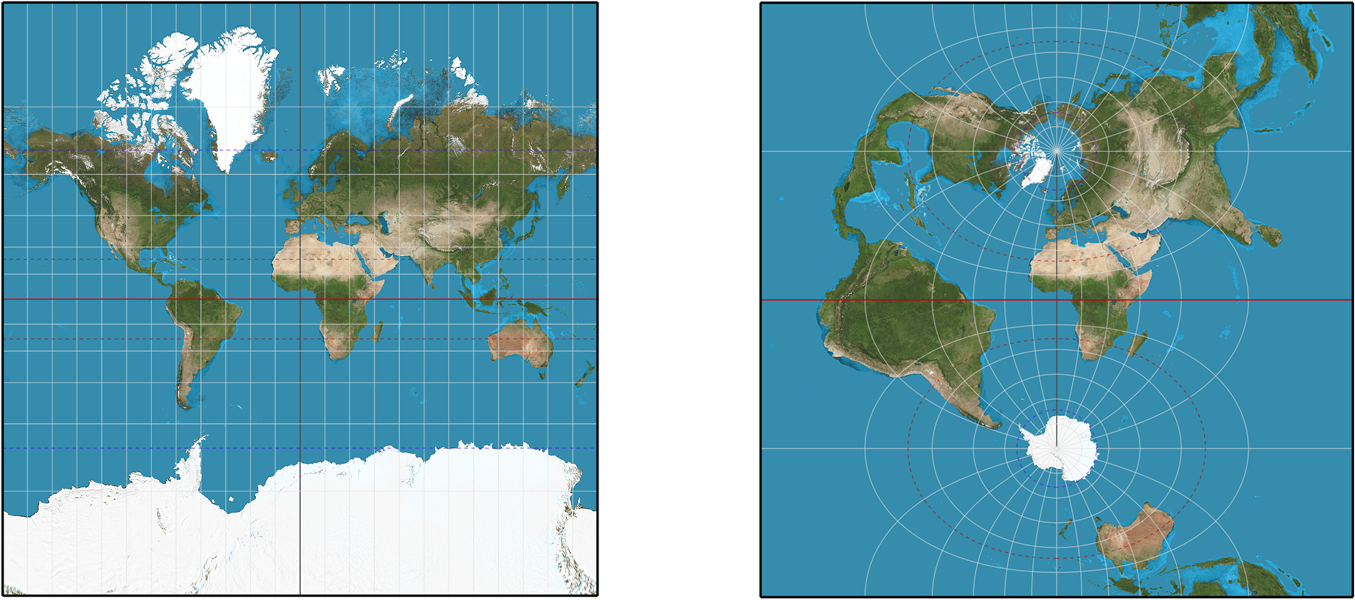
\includegraphics[width=1\textwidth]{res/Mercator}
	\caption{Normal and transverse Mercator projection. \url{https://commons.wikimedia.org/w/index.php?curid=9910866}}
	\label{fig:mercator}
\end{figure}

\subsubsection{EPSG:4326 -- WGS 84}
The most recent version of the Mercator projection is called WGS 84. It improves in accuracy compared to WGS 72 and is an \enquote{European Petroleum Survey Group} (EPSG) standard called EPSG:4326, created by \cite{Decker1986}.\\
WGS 84 is an ellipsoidal coordinate system that shows the 3D surface of the earth in 2D. The coordinates are longitude and latitude measured in degree. Longitude has the 0° point in Greenwich, England and increases east to a maximum of 180° and west to a minimum of -180°. Latitude has the 0° point at the equator and increases north to a maximum of 90° and south to a minimum of -90.\\
WGS 84 is used by the Global Positioning System (GPS), GIS specialists, inside the OpenStreetMap (OSM) database, as well as Google Earth.

\subsubsection{EPSG:3857 -- WGS 84 / Pseudo-Mercator}
Pseudo-Mercator is a projected version of WGS 84 into a two-dimensional cartesian coordinate system. It is also referred to as EPSG:3857 and was created by \cite{Grafarend1995}.\\
The CRS is based on a plane, rather than an ellipse. The zero points is identical to WGS 84 but the coordinates are X and Y measured in meters. The Y coordinate is limited to ±85.06° of the WGS 84 bounds. This results in a square projection with a range of ±20,026,376.39m on both axis, but sacrifices the poles to some extend. The square shape allow the creation of tile pyramids, also called \enquote{Mercator Pyramids} to be used for maps in browsers for the web. \\
A pyramid consists of square images in fixed size, e.g. 256x256px. The First level has one image that shows the whole area of the data with minimal detail. On every level below the number of image tiles increases and therefore the level of detail. The number of tiles on a given level is
$$x_n= 4* x_{n-1}$$ 
where \enquote{x} is the number of tiles and \enquote{n} is the current level of detail. Figure \ref{img:mercator-pyramid} shows an example of a Mercator pyramid.
\begin{figure}[H]
	\centering
	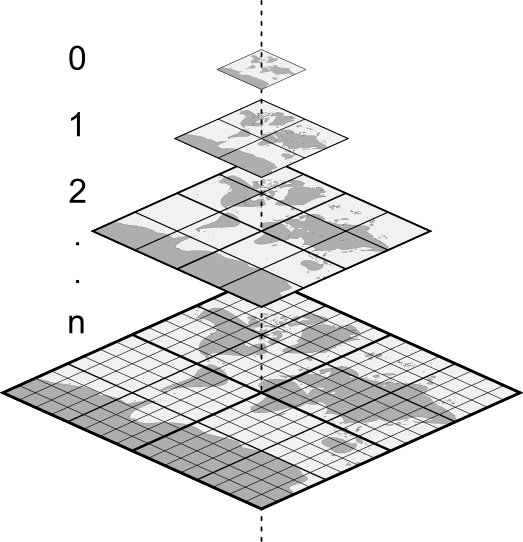
\includegraphics[width=0.4\columnwidth]{res/mercator-pyramid}\\
	\caption[]{Mercator tile pyramid. \url{http://data.webglearth.com/doc/webgl-earthch1.html}}
	\label{img:mercator-pyramid}
\end{figure}
This fragmentation of a big dataset is optimal to be loaded on demand and cached by a web browser, which is why major map sites, like OpenStreetMap, Google Maps and Bing Maps use Pseudo-Mercator as their reference system.


\subsection{Spatial Data Types}
Geo-spatial data exist in two different types, vector and raster. 

\subsubsection{Raster Data}
 Raster data consists of a grid in fixed size. Depending on the file, each pixel contains a color (e.g. satellite data)  or a grayscale (e.g. elevation maps) value.\\
 The advantage of raster data is that it is better suited to store picture like data with gradients. Due to its nature, raster has data in every cell, which leads into a high amount of data that has to be stored, so the potential file size if big.\\
 Since the raster size is fixed, the balance between desired detail and small file size has to be decided upon file creation. Figure \ref{img:raster} shows a shape in three different rasterized resolutions, visualizing the loss of detail.
 \begin{figure}[H]
 	\centering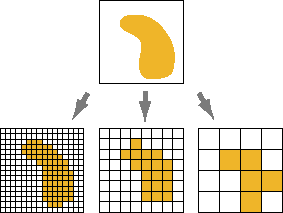
\includegraphics[width=.5\textwidth]{res/Vector-Raster}
 	\caption{Shape as raster in different resolutions. \url{http://desktop.arcgis.com/en/arcmap/latest/manage-data/raster-and-images/what-is-raster-data.htm}}
 	\label{img:raster}
 \end{figure}
Common file types for raster data are GeoTIFF, ESRI, ESRI ArcGrid and ASCIIGrid. GeoTIFF and ArcGrid are binary file types and ASCIIGrid is text-based.

\subsubsection{Vector Data}
In contrary to raster data, vectors files don't map color information to a specific pixel, but define mathematical shapes which are rendered as desired. This allows very efficient storage and it is possible to scale the shapes as desired.\\
Data inside vector GIS can have several layers. Each layer has the type points, line or polygon. The data on a layer is called a feature and matches the layer type. A point feature has a single coordinate (e.g. a well in the ground). Lines are open polygon lines and are used for shapes like walls, streets or rivers. Polygons are closed lines and are used for areas, such as countries, lakes, or larger objects. Figure \ref{img:vector} shows a vector file with the mentioned 3 layers types. The point layer shows the position of wells, the line layer shows a river and the polygon layer a lake.\\
While vector files have the advantage of efficient storage, they have the disadvantage of not being universally usable. The mathematical functions in which data is represented, are not well suited for data without discrete values. Anything that has gradients is better suited for raster.\\
The most common vector file formats are ESRI Shapefile as binary and GeoJSON as a text-based format.

\begin{figure}[H]
	\centering
	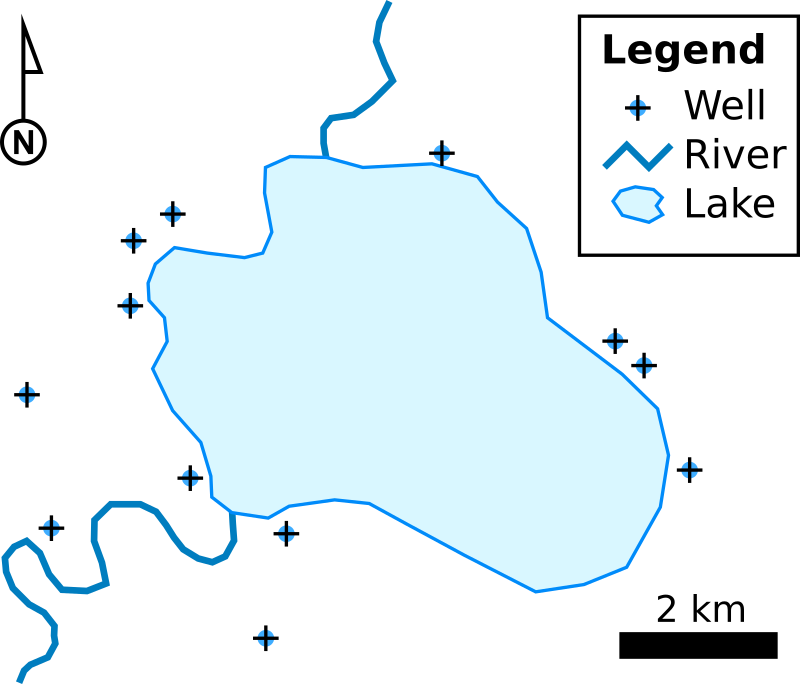
\includegraphics[width=0.4\columnwidth]{res/vector-map}\\
	\caption[]{Vector map with point, line and polygon. \url{https://commons.wikimedia.org/w/index.php?curid=3024482}}
	\label{img:vector}
\end{figure}



\section{GIS Technologies}
This chapter introduces the GIS technologies that were considered for usage during this work. They are grouped into \enquote{spatial databases}, \enquote{GIS Libraries} and \enquote{Others}. Figure \ref{fig:technology_overview} shows a brief overview and compatibility of the libraries.

\begin{table}[H]
	\caption{GIS solutions feature comparison}
	\label{fig:technology_overview}
	\begin{tabular}{|l|l|l|l|}
		\hline \textbf{Name}	& \textbf{Raster support} & \textbf{Vector support} & \textbf{Type}\\
		\hline PostGIS	& Yes* & Yes & PostgreSQL DB + GIS ext.\\
		\hline MongoDB	& No & Yes & NoSQL DB with spatial capabilities\\\hline
		\hline Dotspatial & Yes & Yes & C\# library\\
		\hline NetTopologySuite	& No & Yes & C\# library\\\hline
		\hline GeoServer & Yes & Yes & Self-hosted product\\
		\hline GDAL & Yes & Yes & Library for geospatial manipulation\\
		\hline
	\end{tabular}
	\caption*{ \raggedright * Large file failed.}
\end{table}


\subsection{Spatial Databases}
Spatial databases are DBs that have been extended to store and query spatial data types.

\subsubsection{PostGIS}
PostGIS \citep{Obe2011} is an extender to the object-relational database PostgreSQL \citep{Momjian2001} that allows to store and query both raster and vector GIS. The interaction with the database is done through SQL.\\
PostGIS supports numerous file types for both raster and vector data. The import process is done with specific tools that come as command-line applications which are bundled into the installation. The geometry type allows spatial queries regarding certain areas. These allow to extract single pixel values from raster files as well as feature extraction from vector files. A full list of features can be found at \url{http://postgis.net/features/}.

\subsubsection{MongoDB}
MongoDB is a document-based (NoSQL) database. Data is stored in binary JSON (BSON) and input, as well as output data is in JSON format.\\
As of version 3.4.9 MongoDB supports only vector GIS. It does not support a wide range of format types, but only GeoJSON \citep{Butler2016}. However, it is quite easy to convert the common vector files to GeoJSON using GDAL (see \ref{sec:gdal} for more details).


\subsection{GIS Libraries}
The amount of proper maintained GIS libraries for C\# is very limited. DotSpatial and NetTopologySuite are among the only libraries with community support behind them.

\subsubsection{DotSpatial}
DotSpatial is a GIS library for .Net Framework that allows reading and writing of both raster and vector data. Besides it's manipulation capabilities, it offers functionality for map visualization that allows displaying data. Unfortunately the library has not been ported to .Net Core yet.

\subsubsection{NetTopologySuite (NTS)}
NetTopologySuite is a C\# reimplementation of the JTS Topology Suite (formerly known as "Java Topology Suite"). It is a library for geospatial vector data manipulation. Raster data handling is not supported. The Library has been migrated to support .NET Core in the fall of 2017.


\subsection{Others}
The following technologies did not fit the previous categories. The GeoServer stores and manages GIS yet is not database itself and GDAL is a GIS library which is used as standalone software.

\subsubsection{GeoServer} \label{sec:GS}
The GeoServer is an open source software that is tailored to store, manage and share GIS. It offers a web UI as well as a REST API for interaction. The API is structured in a way that it implements common Open Geospatial Consortium (OGC) standards for retrieving data.\\
The Web Feature Service (WFS) allows to retrieve features of vector data, Web Coverage Service (WCS) enables downloading raster data and the Web Map Service (WMS) can generate a tile map for viewing GIS on a map.
%\\The GeoServer is build for working with few files and a small number of users. The MARS use-case requires to read thousands to millions of single values in parallel in a short amount of time. The GeoServer does not satisfy this demands. The retrieval of single values is not supported, since the general use-case is to work with complete files and the performance for retrieving data is very poor which will require a better solution.\\
%figure \ref{img:gs-read-performance} emphasizes this. It shows GeoServer response time for different storage solutions. All values exceed one second which is not expectable for the amount of requests needed for this work. \cite{Pandey2016} argues that disk-based systems are generally not fast enough for real-time analysis.
%
%\begin{figure}[H]
%	\centering
%	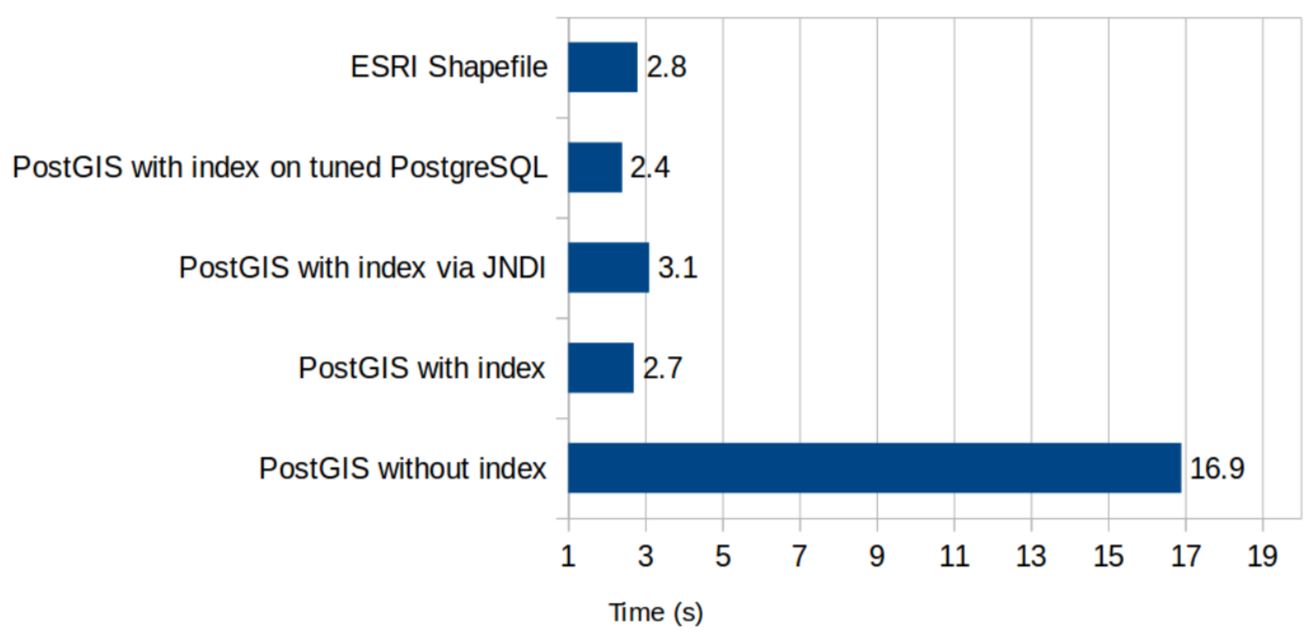
\includegraphics[width=0.8\columnwidth]{res/gs-read-performance}\\
%	\caption[]{GeoServer average time of response by \cite{ruuvzivcka2016comparing}}
%	\label{img:gs-read-performance}
%\end{figure}

\subsubsection{Geospatial Data Abstraction Library (GDAL)}
\label{sec:gdal}
GDAL is a GIS library that is capable of reading and converting various data formats. It current version (2.2.2) supports 142 different raster and 84 vector formats. The library is distributed as a combination of various command-line tools that are each tailored at a specific task. E.g. gdal\_translate converts files between different formates.\\
The gdal tools work with raster data and the ogr tools work with vector data. Ogr stands for \enquote{OpenGIS Simple Features Reference Implementation} and is bundled in the gdal installation.


\section{MARS}
MARS (Multi-Agent Research and Simulation) is a working group at the HAW (University of applied Sciences) in Hamburg, Germany. The research group develops an distributed agent-based simulation system \citep{Wooldridge2009} to be used by domain experts around the world. It consists of several components.


\subsection{LIFE}
The simulation system is called MARS LIFE. It executes simulation. For more detail see \cite{Huning2016}.


%\subsection{Cloud Services}
%The Cloud Services are the central back-end of the MARS system. These components are responsible for data import, persistence, data visualization an the connection between LIFE and the WebUI.
%
%
%\subsection{WebUI}
%The WebUI is the front-end of MARS. It is a web-based application that allows the user to control back-end services and trigger simulations from the web-browser.



\section{C\# Platforms}
The LIFE simulation system is written in the C\# language. There are however differences between the three platforms .NET Framework, Mono and .NET Core which are important for the implementation of this work.


\subsection{.NET Framework}
.NET Framework is the original platform C\# is running on. It is widely used in the industry and is supported by Microsoft. Unfortunately it is Windows only, which is why the community created Mono.

\subsection{Mono}
Mono is an open C\# implementation which is cross platform and therefore also available for Linux and OSX. The implementation of Mono is almost complete which makes most applications that don't require platform specific code like GUI modules on all OS. The implementation of Mono is not build for high performance use-cases like MARS.

\subsection{.NET Core}
In 2016 Microsoft released it's own platform independent .NET version, called .NET Core. It is a complete rewrite of the .NET Framework to satisfy the shortcomings of both alternative solutions.\\
With it's current version (2.0) it has still some missing core functions, which leads to incompatibilities regarding existing software.
